\documentclass[usenatbib]{aastex}
\usepackage{amsmath,amssymb}
%\usepackage{natbib}
%\documentclass{article}
\usepackage{graphicx} 
\begin{document}

\section{Science Justification}
Weak gravitational lensing has been widely touted as a powerful probe of cosmology. It is a major science driver for several large imaging surveys, such as the Dark Energy Survey (DES) the Large Synoptic Survey Telescope (LSST), and space missions such as Euclid and the Wide-Field Infrared Survey Telescope (WFIRST). Weak lensing is weak, however, and all current measurements are limited by the scatter in galaxy shapes, which is an order of magnitude or more greater than the typical weak lensing signal. This means that weak lensing analyses must average over every available galaxy image, pushing the analysis to include faint and poorly-resolved galaxies for which unbiased measurements of galaxy shapes are difficult. Precision estimates of galaxy redshifts from photometry is crucial for these analyses, as the current generation of ongoing surveys will entail sample sizes of a few $\times10^8$ galaxies, which is two orders of magnitude beyond the size of the largest existing spectroscopic samples. Percent-level biases in the photometric redshifts will have a large impact on the error budgets for this next generation of surveys.

Here we propose a pilot study for a new weak lensing measurement technique that avoids many of the above problems, and promises a very large reduction in the effective lensing noise. The velocities and 

\begin{figure}[t]
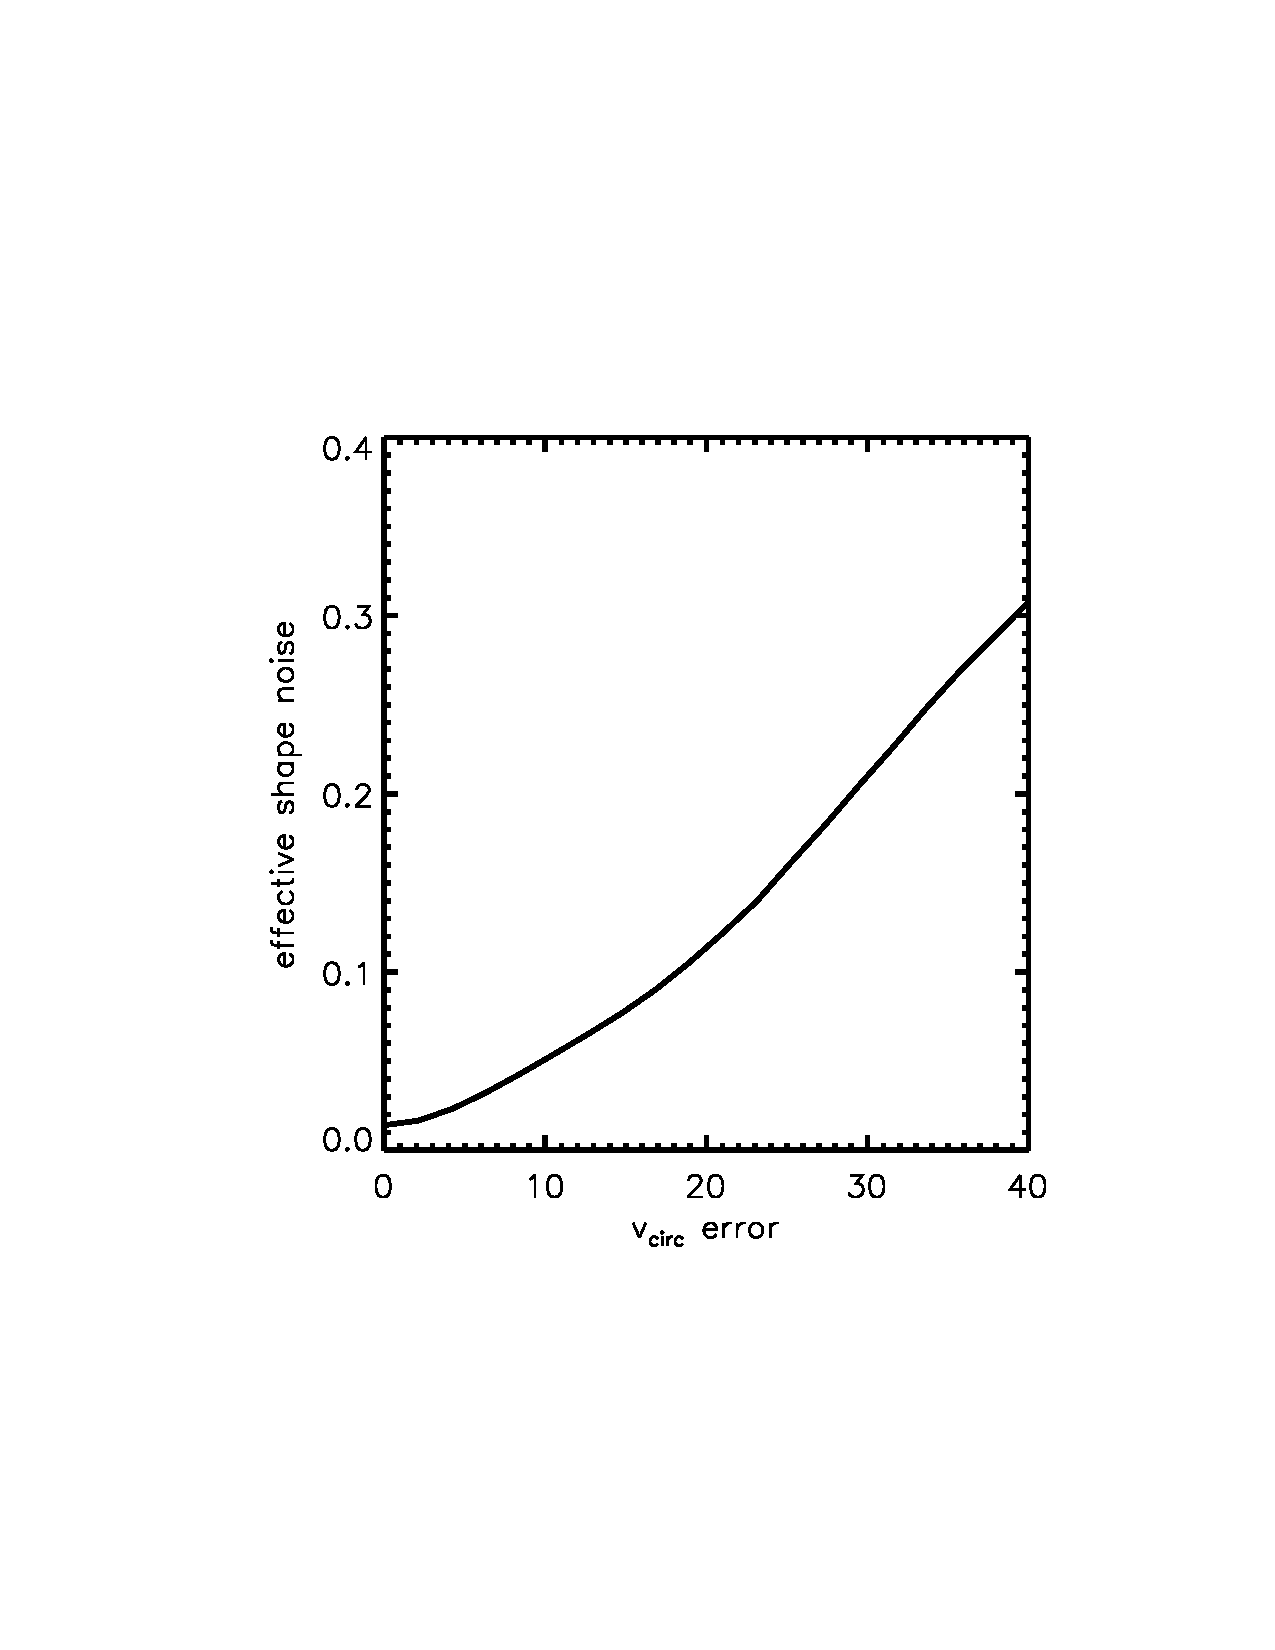
\includegraphics[width=\linewidth, bb= 150 150 550 650,clip]{Plots/vcirc_error.pdf}
\caption{Effective shape noise $\sigma_{TF}$ as a  function of the
  measurement error on the disk circular velocity.}
\label{fig:shapeNoise}
\end{figure}

\subsection{}


\subsection{A Pilot Study for a Stage V Dark Energy Experiment}

\end{document}